\chapter{Server}
\label{server}

Server associate all connected clients and it is enabling mutual communication. Server is able to request authentication by name and password or by token.

\section{Client}

Each connected client is virtually represented on server by unique ID on interval $0$ to $2^{32} - 1$ and it's user name (nick). User name can be duplicate on server (only ID has to be unique).

\section{Rooms}

Server contains rooms, this rooms cam be used to mutual communication among joined users. Server is able to maintain zero to $2^{32}$ rooms (limitation of 4 bytes length ID). Each room has own ID and name. Room can be opened or locked by password.

Clients can communicate together just in case that there are in same room. Every client is outside of all rooms after connection to server. Single client can be only in one room simultaneously therefore client can join room just in case that it is not in other room in that time. Clients can joint (connect to), leave and create rooms. When client create new room it is automatically connected to this new room. Room exists just if there is at least one client, otherwise room is destroyed. See figure \ref{server.pictures.server_client_rooms} for illustration.

\begin{figure}[h]
  \centering
  \includegraphics[width=0.80\textwidth]{diagrams/server_client_rooms.png}
  \caption{Clients, server and rooms}
  \label{server.pictures.server_client_rooms}
\end{figure}

\subsection{Canvases and layers}

The main target of the protocol is shared drawing. It is maintained (in rooms) by canvases and layers. Each room can contain several canvases and each canvas can contain layers. Canvas is composed by layers which user can draw into. Structure of room is illustrated by figure \ref{server.pictures.room}.

\begin{figure}[h]
  \centering
  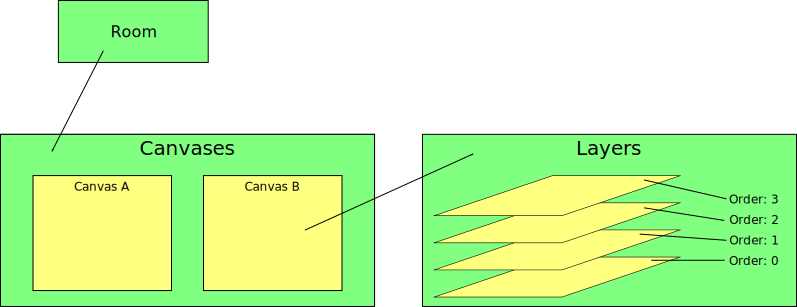
\includegraphics[width=0.80\textwidth]{diagrams/room.png}
  \caption{Room}
  \label{server.pictures.room}
\end{figure}

Every canvas has own dimension (in pixels), name and ID. There is no specified order of canvases it is depends just on client. Layers have particular order specified by server.

Room can contain $0$ to $2^{32}$ (4 bytes ID) canvases and canvas is composed of $0$ to $2^{32}$ layers.

Canvas has owns ID, order.

Layer is picture with $32$ bits color depth -- 1\,{}B is used for alpha channel (opacity).

Order of layers starts with $0$ and ends with $p - 1$ where $p$ is count of layers in canvas. Layer with order $0$ is under all other layers, controversially layer with list $p - 1$ is painted over rest of layers. General rule is that order is number of layers painted under this particular layer. See figure \ref{server.pictures.room}.

\subsection{Chat}

Chat is cherished inside of rooms.  Clients outside of all rooms can't chat with anybody!

\subsection{Another services}


